\section{Admitting a new domain}
\label{app:admit}

\slowlab{} is a harness for a class of problems rather than for one domain. A domain is
admissible when it supplies four things.

\emph{The conditions must hold jointly and by nature}, not because the benchmark author chose
hyperparameters that way (\S\ref{sec:domain}).

\emph{A published forward model} must exist, so that the response surface, its noise
structure and the location of its optimum are fixed outside the benchmark author's control.

\emph{A cost model in the objective's own units} must be available, so that exploration is
priced rather than constrained from outside.

\emph{Experimental units must not be interchangeable.} Some structure---blocks, batches,
chambers, cohorts---must constrain which treatments can be assigned where, because that is
what makes allocation a decision rather than bookkeeping, and what makes replication compete
with coverage.

\paragraph{}
Greenhouse horticulture, the instantiation built here, satisfies all four
(\S\ref{sec:domain}). Microbial evolution experiments, bioprocess scale-up, materials
ageing and dose-finding trials meet them with published forward models already in hand. We
do not claim results transfer across domains---that is the question a multi-domain version
would exist to answer---only that the harness, the measures and the reference points are
defined at the level of the class.

\paragraph{Four extensions that need no environment code.} The crop model already contains
the mechanism each of them tests, so each is a task specification. \emph{Equipment faults}
give ground-truth attribution: a heater fails in one chamber for $k$ days, the agent sees an
unexpectedly low yield and an anomalous log, and must name the cause, which is exact because
we injected it. \emph{Fruit abortion} above $T_{\mathrm{CRIT}}$ already makes irreversibility
graded rather than binary, from recoverable through partially recoverable to a terminated
unit. \emph{Between-season parameter drift} within the published between-site spread makes
conclusions expire on a schedule the data rather than we set. And because the oracle is
computable in a tenth of a second, a \emph{target profit rate} sorts instances into
comfortably feasible, feasible only in a narrow region, marginally infeasible and clearly
infeasible, which tests whether an agent can recognise that it has been asked for something
impossible. None of these can be built on a surrogate without injecting the abstraction by
hand.

\section{A worked round}
\label{app:worked}

Figure~\ref{fig:worked} runs one round of \textsc{Optimise} through in full: one site, one
twelve-unit budget, two designs that both pass the feasibility check and differ only in how
the units are allocated. It is the smallest case in which the control hierarchy of
\S\ref{sec:facility} decides the answer, and the reason the environment scores allocation
rather than treatment choice alone.

\begin{figure}[h]
\centering
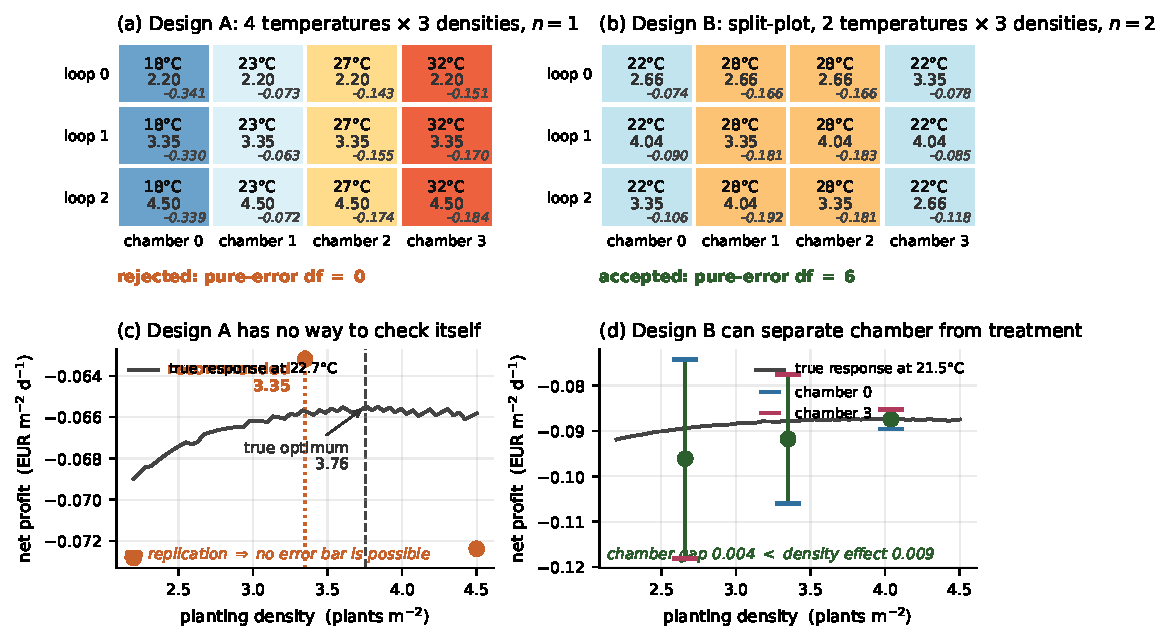
\includegraphics[width=\linewidth]{figures/fig2_worked_example.pdf}
\caption{One round of the running scenario: same site (\texttt{seed=0}), same twelve-unit
budget, two designs. All values are produced by the environment; the script is in the
repository. \textbf{(a)} The intuitive design fills the grid---four temperatures, one per
chamber, crossed with three densities. It passes \texttt{validate\_design}, but every
treatment is observed once, so pure-error df is zero and each temperature is confounded
with one chamber. \textbf{(b)} The split-plot: two temperatures, each replicated across two
non-adjacent chambers, densities randomised within chamber. Our first attempt used chambers
0--1 and 2--3 and was rejected by the randomisation check---temperature then correlates
perfectly with chamber index. \textbf{(c)} Design A's best observation sits at $3.35$ plants\,m$^{-2}$ where the true
optimum at that temperature is $3.76$; the miss is small, and the point is that with one
observation per treatment nothing in the data says whether it is small. \textbf{(d)}
Design B can answer the question it was given: the chamber 0 against chamber 3 gap at
identical settings is $0.004$ against a density effect of $0.009$, so the effect is
resolvable above the block noise --- which is a statement design A cannot make either way.
The figure is regenerated from the frozen environment; an earlier version hard-coded the
annotations and printed the comparison in (d) with the inequality facing the other way.}
\label{fig:worked}
\end{figure}


\section{Task specifications}
\label{app:tasks}

\begin{table}[h]
\centering\small
\begin{tabular}{@{}llll@{}}
\toprule
\textbf{Factor} & \textbf{Range} & \textbf{Control level} & \textbf{Role} \\
\midrule
day temperature   & 18--32\,\textdegree C     & chamber & heating/ventilation setpoint \\
night temperature & 12--22\,\textdegree C     & chamber & setpoint \\
CO$_2$            & 350--1200\,ppm            & chamber & enrichment \\
PAR               & 18--32\,mol\,m$^{-2}$d$^{-1}$ & chamber & natural + supplemental \\
plant density     & 2.2--4.5\,m$^{-2}$        & loop    & planting decision \\
$\mathrm{LAI}_{\max}$ & 2.0--5.0              & loop    & pruning target \\
\bottomrule
\end{tabular}
\caption{The six management factors. Control level is a physical fact---lamps and heating
serve a whole chamber, whereas density and the pruning target are set per hydroponic
loop---and it determines each factor's parallelism ceiling.}
\end{table}

The noise column of Table~\ref{tab:tasks} is
\[
  \sigma_{\mathrm{tot}}/\sqrt{B} \;=\;
  \sqrt{\mathrm{sd}^2\Big(\tfrac{\tau_{\mathrm{loop}}^2}{B}
  + \tfrac{\tau_{\mathrm{chamber}}^2}{CR} + \tfrac{\tau_{\mathrm{batch}}^2}{R}\Big)},
\]
the standard error of the mean of $B = R \times |\mathcal{U}_r|$ observations spread over
$C$ chambers and $R$ rounds. Only the first term falls with $B$: a chamber effect is shared
by every unit in that chamber and a batch effect by every unit in that round, so past a
point buying more units stops buying precision. That is the width constraint of
\S\ref{sec:conditions} in arithmetic.

Two quantities a grower does control are declared by the task rather than exposed as
factors, and the environment refuses to treat either as one. Cycle length is fixed at
$210$ days: it is monotone over any plausible range, because fruit set does not begin until
roughly 30--45 days and that establishment period is pure cost, so exposing it would add a
dimension with the same answer at every site. Leaf removal is fixed at
$2.25$\,g\,node$^{-1}$ because the reduced model gives defoliation no photosynthetic
penalty, so its optimum is always at the upper rail. Both are asserted rather than
silently overridden, so anyone who adds them back gets an error instead of a sweep that
quietly holds them constant.

\section{The naive corner}
\label{app:naive}
Setting every factor to its upper bound yields \emph{negative} profit at every site,
worse than the site optimum by a factor of $4$ to $52$; setting every factor to its
midpoint is also negative at most sites, worse by a factor of $1.3$ to $21$. Maximising everything fails because day temperature at its ceiling aborts fruit set
(eq.~8) while supplemental lighting continues to draw power. We use this rather than
``every factor has an interior optimum'' as the criterion for a non-trivial search problem.

\section{Reproducibility}
\label{app:repro}
All results use seeds $0..N{-}1$; \texttt{SlowLabEnv(task, seed)} is deterministic, and the
seed selects a sampled site rather than only a noise realisation. Every table and figure in this paper is emitted by a script in \texttt{scripts/} from
the JSON under \texttt{results/}, and none is hand-edited. The files carry the environment
version in their names, so a table built from a previous environment cannot be picked up
silently. Code, task definitions and those scripts are released under the MIT licence at
\url{\projecturl}. The $800$ raw language-model transcripts and the cached atom sets are
published there as a release asset rather than in the repository itself.
\todo{datasheet, croissant metadata, hosting}

\section{The $\mathcal{R}^\star$ estimator}
\label{app:eig}

\paragraph{Observation likelihood.} Because the per-unit draw $\phi_u$ is pushed through the
forward model, $p(y \mid \theta, x)$ has no pointwise density. We moment-match the per-unit
response to a Gaussian with variance $s^2(x)$, which makes the covariance of a round's
$|\mathcal{U}_r|$ observations
\[
\Sigma(D_r) \;=\; \operatorname{diag}\!\big(s^2(x_u) + \tau_\gamma^2\big)
\;+\; \tau_\beta^2\, Z Z^{\!\top} \;+\; \tau_\epsilon^2\, \mathbf{1}\mathbf{1}^{\!\top},
\]
with $\tau_\beta, \tau_\gamma, \tau_\epsilon$ the nuisance scales of \S\ref{sec:conditions}
and $Z \in \{0,1\}^{|\mathcal{U}_r| \times C}$ the block-membership matrix. The allocation
enters through $Z$, so where a design places its treatments changes
\eqref{eq:eig}, not only which treatments it chooses.

\paragraph{Three approximations.} \emph{(a)} The Gaussian moment-match above.
\emph{(b)} $s^2(\cdot)$ is computed once at the nominal parameter vector rather than per
atom. \emph{(c)} The prior is the $M$-atom mixture rather than the continuous $P_\Theta$.
We had argued that (c) was benign, on the grounds that the dimension which matters is that
of $x^\star_\theta$ rather than of $\theta$, and that it is small --- over $150$ instances
of \textsc{Optimise} the true optima occupy ten grid cells at
$H\big[p(x^\star_\theta)\big] = 2.05$ nats. That argument is wrong, and the next two
paragraphs are what it cost. The support of $x^\star_\theta$ being small does not make the
\emph{likelihood} over atoms well behaved, and it is the likelihood that fails.
\pending{Moment diagnostics for (a) and (b).}

\paragraph{The in-sample estimator and why we abandoned it.} Our first estimator drew one
atom set and used it for everything: the posterior weights $w_m(y)$, the minimisation over
candidate recommendations, and the evaluation of the chosen recommendation. The failure is
mechanical. $\Sigma(D_r)$ above contains observation noise and block structure and nothing
for the coarseness of the grid, so with $12$ to $24$ observations the likelihood
discriminates between atoms far more sharply than the grid spacing warrants. Measured over
$160$ atoms on \textsc{Optimise}, the mean effective sample size $1/\sum_m w_m^2$ is
$1.1$, and the candidate that minimises $w^{\!\top}\!D$ is some atom's own optimum in
$98\%$ of draws. The estimator was therefore answering ``can the data identify which of
these $160$ sites generated it'' and reporting the answer as though it were ``how much
decision risk does this design remove''. Held out on atoms that did not generate the data,
the same designs score $c = -64\%$ where the in-sample number reads $+97\%$: conditioning on
the design leaves the reasoner worse than the prior-optimal constant, because the posterior
concentrates on a wrong atom and the recommendation follows it there.

\paragraph{The estimator we report.} Three changes, all in
\texttt{achievable\_regret\_cv}. The likelihood is raised to the power $1/T$, equivalently
$\Sigma \to T\Sigma$, which is the minimal way to state that the true site lies between
atoms. $T$ is selected by leave-one-out over the inference atoms: for each atom $m$, draw
$y$ from $m$, form the posterior from the others, choose a recommendation, and score it at
$m$; take the $T$ minimising the average. The evaluation atoms are never touched, so
selecting $T$ cannot import the bias it removes, and the leave-one-out curve tracks the
held-out curve closely enough to be used as its proxy. Finally the recommendation is scored
on the disjoint half. The result is $c$ between $1\%$ and $20\%$ where the in-sample
estimator read $35\%$ to $78\%$, and the orderings differ: on \textsc{Optimise} the
in-sample estimator ranked random search first among the reference strategies and the
repaired one ranks it last.

We tried the obvious cheaper fix first. Fitting the surrogate hyperparameters is not it and
neither is raising $M$ alone; tempering is what moves the number, and the temperature the
calibration selects is $3$ to $100$, meaning the effective observation covariance is one to
two orders of magnitude larger than the noise model alone implies. That is the size of the
discretisation error, stated in the only units available.

\paragraph{Convergence in the atom count.} Table~\ref{tab:conv} runs seven designs at
$M = 80$ and $M = 320$ on the two tasks we could afford at both counts, six runs each. The
designs span the range of $c$ rather than compete: space-filling, a two-level factorial,
four, two and one distinct treatments, and the two degenerate cases of every unit at a
corner and every unit at the centre.

The estimator has not converged and the direction of its error is now the opposite of the
in-sample one. Quadrupling $M$ leaves the degenerate designs where they are and lifts the
good ones: on \textsc{Screen} the space-filling design goes from $0.8\%$ to $16.5\%$. The
reason is the split. At $M = 80$ only $40$ atoms carry the posterior, which is too coarse a
stand-in for $P_\Theta$ for any design to separate, so the measure reports that no design
helps. Every level we report is therefore a lower bound on what a converged estimator would
give, which is the conservative direction for claims of the form ``no agent reaches the
ceiling'' and the awkward one for any claim that a particular agent's design was poor.

Rank correlation between the two counts is $0.82$ on \textsc{Optimise} and $0.64$ on
\textsc{Screen}. That is lower than the in-sample estimator reported and it is the honest
number: the in-sample estimator's near-perfect rank stability was itself an artefact, since
a posterior that always collapses onto one atom is a deterministic function of design
geometry and therefore stable in $M$ for the wrong reason. A single estimate carries a
standard deviation of $2$ to $4$ points. Every $c$ in this paper is a mean over dozens of
designs, where that falls below one point, and the comparisons we draw conclusions from are
paired at fixed $M$.

\begin{table}[h]
\centering\small
\begin{tabular}{@{}lcccc@{}}
\toprule
& \multicolumn{2}{c}{\textsc{Optimise}} & \multicolumn{2}{c}{\textsc{Screen}} \\
\cmidrule(lr){2-3}\cmidrule(lr){4-5}
\textbf{Design} & $c$ at $M{=}80$ & $M{=}320$ & $c$ at $M{=}80$ & $M{=}320$ \\
\midrule
space-filling & $21.7\pm1.3$ & $29.6\pm2.0$ & $0.8\pm0.9$ & $16.5\pm0.8$ \\
four treatments & $2.2\pm1.6$ & $16.0\pm1.4$ & $0.5\pm1.1$ & $7.8\pm0.8$ \\
two treatments & $4.4\pm1.5$ & $12.2\pm1.5$ & $12.9\pm0.9$ & $7.8\pm1.1$ \\
two-level factorial & $-2.0\pm1.8$ & $-0.5\pm2.1$ & $-1.7\pm0.4$ & $3.4\pm1.1$ \\
corner only & $-1.9\pm1.5$ & $-1.7\pm2.1$ & $0.7\pm0.8$ & $1.5\pm0.8$ \\
centre only & $-0.4\pm1.6$ & $-1.9\pm1.7$ & $-0.4\pm1.3$ & $-3.1\pm0.5$ \\
one point & $-2.0\pm1.6$ & $-2.3\pm2.1$ & $-0.7\pm1.1$ & $0.6\pm0.6$ \\
\midrule
\multicolumn{5}{@{}l}{$\mathcal{R}^\star(\varnothing)$: \textsc{Optimise} 0.00546 $\to$ 0.00610; \textsc{Screen} 0.00500 $\to$ 0.00443} \\
\multicolumn{5}{@{}l}{rank correlation of $c$ between the two atom counts: $0.82$ and $0.64$} \\
\bottomrule
\end{tabular}
\caption{Design efficiency at two atom counts under the cross-validated estimator, seven designs chosen to span the range rather than to compete. Each entry is the mean of six independent runs with its standard error; a single run carries a standard deviation of $2$ to $4$ points, which is why the levels reported elsewhere in this paper are always means over dozens of designs. Quadrupling the atom count leaves the two degenerate designs where they were and roughly doubles the best one on \textsc{Optimise}; on \textsc{Screen} it moves the space-filling design from nothing to the top. The estimator is not converged, and the direction of its error at low $M$ is to under-credit good designs, because half of $80$ atoms is too coarse a stand-in for $P_\Theta$ for any design to separate.}
\label{tab:conv}
\end{table}


\paragraph{The bound does not survive estimation.} For the exact quantities $c \in [0,1]$
is a theorem: numerator and denominator start from the same beliefs, so
$\mathbb{E}[\min] \le \min[\mathbb{E}]$ gives $\mathcal{R}^\star(D_r) \le
\mathcal{R}^\star(\varnothing)$, and $\mathcal{R}^\star \ge 0$ closes the other end. The
estimator above is a tempered rule graded out of sample, about which the optimality theorem
says nothing, and the difference is visible: across the $320$ reference rounds behind
Table~\ref{tab:refs}, $69$ carry a negative $c$. Averaged over the dozens of rounds that
make up one cell every value we report is inside $[0,1]$ --- $c$ from $1\%$ to $20\%$,
$\eta$ from $4\%$ to $56\%$ --- but by margin rather than by proof. For $\eta$ there is
not even an exact bound to appeal to, since the agent's $\hat{x}_r$ has seen every round
while the numerator scores each round separately against the prior.

\paragraph{Trajectory and endpoint.} The interim recommendation elicited after each round uses
the same rule the agent applies at the end, so the last point of a trajectory equals the
regret of the submitted recommendation. This is asserted by a regression test: an earlier
version used the best observed point for the trajectory and a posterior maximum for the
submission, which differed by $47\%$ on \textsc{Optimise}.

\section{The horticultural instantiation}
\label{app:domain}

\paragraph{Forward model.} $f_\theta$ is the reduced state-variable TOMGRO model
\citep{jones1999reduced}: five coupled state variables---mainstem nodes, leaf area index,
above-ground, fruit and mature-fruit dry weight---implemented from its equations (1)--(11)
with the published least-squares estimates. We deliberately do not sample ground truth from
a Gaussian-process prior: such a sample has no physical content, its length scale would be
our choice, and it makes the modelling assumption of GP-based agents exactly correct.
Fitting our Bayesian-optimisation reference's own surrogate to the mechanistic response
gives mean absolute error $1.1\times$ the global average in the high-temperature decline and
$2.2\times$ near the kink where supplemental lighting begins to incur cost---real but mild,
and the surrogate still locates the optimum. What the mechanistic surface supplies that a
stationary GP cannot is structure: fruit abortion above $T_\mathrm{CRIT}$ (eq.~8), the
source of irreversibility, and a source--sink limit taking the \emph{minimum} of two growth
expressions (eqs.~9--10). $P_\Theta$ follows the same paper's finding that vegetative
parameters are stable across sites while fruit parameters vary: each seed draws fruit
parameters across the published between-site spread ($N_{FF}$ varies by $2.2\times$ across
their three sites). Five of the six factors have optima that move across sites; the sixth,
supplemental light, sits at the lower rail in every instance because at 2024 European
electricity prices it never repays its energy.

\paragraph{Facility.} Blocks are climate chambers and units are hydroponic loops. Lamps,
heating and CO$_2$ enrichment are set per chamber; planting density, pruning target and
the pruning target is set per loop. Cycle length is fixed at $210$ days for every unit and
is not a decision (\S\ref{sec:tasks}).

\paragraph{Costs.} Revenue is fruit fresh weight at wholesale price; costs are supplemental
lighting, heating and CO$_2$ enrichment, computed with standard greenhouse engineering
relations. Coefficients come from public sources rather than from us, because the
\emph{Costly} measure is denominated in euros and an uncited coefficient makes its absolute
value uninterpretable: crop price 1.50~EUR/kg fresh weight, between Dutch (1.57) and Spanish
(1.35) vine tomato in March 2024 \citep{tomato_prices}; electricity 0.189 and natural gas
0.0605~EUR/kWh, the EU non-household averages for 2024 \citep{eurostat_energy_prices};
luminaire efficacy 2.5\,\textmu mol\,J$^{-1}$, the level over half of listed horticultural
fixtures reach \citep{dlc_qpl}; a cover heat-transfer coefficient of
4.0\,W\,m$^{-2}$K$^{-1}$, between single glass ($\approx$4.5) and double polyethylene
(2.9--3.4) \citep{kittas_covers}. The CO$_2$ leakage coefficient yields 14.6\,kg\,m$^{-2}$
per season, inside the 12--24 range that must be delivered for tomato \citep{ahdb_co2}.

\paragraph{Caveats.} The figures are representative European values, not measurements from
one facility. Outdoor temperatures correspond to the Mediterranean--subtropical winters of
TOMGRO's calibration sites rather than to northern Europe, where greenhouses consume
47--69\,m$^3$ of gas per m$^2$ per year ($\approx$460--670\,kWh) against about 245
here---a difference of climate rather than of coefficients. And one consequence was not our
choice: at these prices supplemental lighting is never economical in this climate, so the
optimum for PAR sits at its lower bound for every site.

\section{Scripted references, and how far they get}
\label{app:refs}

Four scripted strategies ship with the environment: random search over the factor space; a
planned campaign, being a Plackett--Burman screen with centre points followed by a response
surface, replicated and randomised across chambers; and Bayesian optimisation at one and at
two replicates per treatment. Table~\ref{tab:refs} runs all four on all four tasks, eight
instances each. They are a reference point, not a baseline we claim to have tuned: each is
a textbook method implemented straightforwardly, and the numbers below say what such an
implementation achieves at these budgets, not what the method is capable of.

\begin{table}[t]
\centering\small
\begin{tabular}{@{}llcccccc@{}}
\toprule
\textbf{Task} & \textbf{Strategy} & $\bar{\mathcal{R}}(R)\downarrow$ & $\mathcal{R}_{\mathrm{cum}}\downarrow$ & $c\uparrow$ & $\eta\uparrow$ & design & decision \\
 & & final answer & campaign cost & & & rank & rank \\
\midrule
\multicolumn{8}{@{}l}{\textsc{Sanity} \quad \small $\mathcal{R}^\star(\varnothing)=0.0055$} \\
& Random search & 0.0417(119) & 345 & 1\% & 13\% & 3 & 4 \\
& Planned campaign & 0.0089(33) & 140 & 9\% & 56\% & 1 & 1 \\
& Bayesian opt.\ (1 rep) & 0.0172(73) & 289 & 1\% & 32\% & 3 & 3 \\
& Bayesian opt.\ (2 rep) & 0.0128(49) & 288 & 5\% & 41\% & 2 & 2 \\
\addlinespace
\multicolumn{8}{@{}l}{\textsc{Screen} \quad \small $\mathcal{R}^\star(\varnothing)=0.0044$} \\
& Random search & 0.0585(92) & 1061 & 20\% & 6\% & 1 & 1 \\
& Planned campaign & 0.0989(84) & 972 & 5\% & 4\% & 4 & 3 \\
& Bayesian opt.\ (1 rep) & 0.0586(183) & 799 & 16\% & 6\% & 2 & 1 \\
& Bayesian opt.\ (2 rep) & 0.0785(188) & 844 & 12\% & 5\% & 3 & 2 \\
\addlinespace
\multicolumn{8}{@{}l}{\textsc{Optimise} \quad \small $\mathcal{R}^\star(\varnothing)=0.0061$} \\
& Random search & 0.0258(82) & 709 & 3\% & 23\% & 3 & 4 \\
& Planned campaign & 0.0251(98) & 510 & 3\% & 24\% & 3 & 3 \\
& Bayesian opt.\ (1 rep) & 0.0120(37) & 496 & 6\% & 48\% & 1 & 2 \\
& Bayesian opt.\ (2 rep) & 0.0107(37) & 540 & 5\% & 54\% & 2 & 1 \\
\addlinespace
\multicolumn{8}{@{}l}{\textsc{Transfer} \quad \small $\mathcal{R}^\star(\varnothing)=0.0041$} \\
& Random search & 0.0706(51) & 2404 & 17\% & 5\% & 1 & 4 \\
& Planned campaign & 0.0653(81) & 1592 & 8\% & 6\% & 4 & 3 \\
& Bayesian opt.\ (1 rep) & 0.0335(36) & 1418 & 13\% & 11\% & 3 & 1 \\
& Bayesian opt.\ (2 rep) & 0.0534(152) & 1644 & 15\% & 7\% & 2 & 2 \\
\addlinespace
\bottomrule
\end{tabular}
\caption{Reference strategies, environment v1.0.0, eight instances per task. $\bar{\mathcal{R}}(R)$ is the regret of the final recommendation, with its standard error in the last two places; $\mathcal{R}_{\mathrm{cum}}$ is the profit the campaign forwent, in \euro\,per square metre summed over committed unit-days. $c$ is design efficiency against the $\mathcal{R}^\star(\varnothing)$ printed above each block. Rank $1$ is best and tied values share a rank; decision rank orders $\eta$, whose levels are in Appendix~\ref{app:eig}. We draw conclusions from the ranks rather than the levels, for the reason given in \S\ref{sec:estimator}.}
\label{tab:refs}
\end{table}


\paragraph{What is and is not tuned.} The Bayesian-optimisation reference uses a
hand-rolled Gaussian-process surrogate whose length scale and observation noise are fixed
rather than fitted, and the tool arm of \S\ref{sec:results} hands the same routine to a
language model. We assumed the fixed hyper-parameters were costing it and checked
(\texttt{scripts/tool\_hyper\_control.py}): refitting length scale and observation noise by
marginal likelihood on exactly the same observations, holding the recommendation rule and
everything else constant, changes the regret of the point proposed by $-25\%$ on
\textsc{Optimise}, $-6\%$ on \textsc{Screen}, $-5\%$ on \textsc{Transfer} and $+32\%$ on
\textsc{Sanity}: better on three tasks, worse on one, and still several times the regret
the same routine carries when it chooses its own designs. The fixed hyper-parameters are
not what limits either. The planned campaign's screen is full
rank over the factors it varies, which is the only property we checked. Both are released
so that a reader can improve on them.

\paragraph{The two efficiencies come apart on \textsc{Transfer}.} Random search ranks
first on design there and last on decision: it spreads its units over the whole space, so
its observations locate the optimum better than any other strategy's, and it then
recommends close to the best point it happened to run. Bayesian optimisation is the mirror
image, concentrating units near the incumbent and converting far more of what that carries.
On \textsc{Screen} the same pattern holds weakly. It does \emph{not} hold on
\textsc{Optimise}, where the repaired estimator puts all four strategies between $3\%$ and
$6\%$ and the task no longer separates designs at all; the in-sample estimator reported
$39\%$ to $46\%$ there and ranked random search first, and that was an artefact. On
\textsc{Sanity} the planned campaign leads on both, which is what a control should look
like. The stronger demonstration that the two measures are not restatements of each other
is in \S\ref{sec:results}, where one intervention moves them in opposite directions within
a single model.

\paragraph{Where the ratio is thin, nothing converts.} On \textsc{Screen} all four
strategies convert between $4\%$ and $6\%$, so the decision column there is close to two
tied pairs rather than an ordering. This is Table~\ref{tab:tasks}'s ratio of $1.5$
restated: when the room for tailoring is barely above what a full budget resolves, the
difference between a good and a bad reading of the data is not detectable.

\paragraph{A screen presumes a campaign these budgets do not pay for.} On \textsc{Screen}
the planned campaign has the worst realised regret of the four, worse than random search,
although its screening design is full rank over the six factors it varies, replicated and
randomised across chambers. At this budget it spends half its units establishing which
factors matter and the other half on a response surface around a noisy incumbent, while
random search spends everything on coverage. Plackett--Burman was designed for a programme
with a follow-up; two rounds are not one.

\section{How much of the ceiling any design can remove}
\label{app:oracle}

\S\ref{sec:results} reports design efficiency without saying what value of it is
attainable, and a reader is entitled to ask whether a small $c$ measures the agent or the
task. If no admissible design can push $\mathcal{R}^\star(D)$ far below
$\mathcal{R}^\star(\varnothing)$, the denominator of \eqref{eq:capture} carries no
information and a low score says only that the problem is hard.

We answer by searching the admissible set directly
(\texttt{scripts/oracle\_design.py}). The search reads $P_\Theta$ and the forward model, so
it is not an agent and its designs are not achievable by one: it is an upper bound on what
the design half of the score could ever report. The set is discrete and hierarchical ---
chamber-level factors take one value per chamber --- so a round is a choice of how many
chambers, how many loops in each, how many distinct chamber-level and loop-level settings,
and where those settings sit in the factor space. We enumerate that grid over five standard
point families (maximin, Latin hypercube, two-level corners, three-level grid, uniform),
check every candidate through the environment's own validator, and score it with the
cross-validated estimator of \S\ref{sec:estimator}. Being an enumeration over families
rather than a proof of optimality, the $c_{\max}$ of Table~\ref{tab:oracle} is itself a
lower bound on the true maximum.

\begin{table}[h]
\centering\small
\setlength{\tabcolsep}{5pt}
\begin{tabular}{@{}lccccccc@{}}
\toprule
& & \multicolumn{2}{c}{\footnotesize best design found} & \multicolumn{2}{c}{\footnotesize best $c$ achieved} & \multicolumn{2}{c}{\footnotesize median $c$ at} \\
\cmidrule(lr){3-4}\cmidrule(lr){5-6}\cmidrule(lr){7-8}
\textbf{Task} & $\mathcal{R}^\star(\varnothing)$ & $c_{\max}$ & $k$ & model & scripted & $k=2$ & $k \ge d{+}1$ \\
\midrule
\textsc{Sanity}   & 0.0055 & $31.7\%$ & 3 & $11.5\%$ & $9.2\%$  & $1.4\%$ & $5.3\%$ \\
\textsc{Screen}   & 0.0044 & $27.8\%$ & 5 & $7.1\%$  & $20.0\%$ & $2.0\%$ & $10.7\%$ \\
\textsc{Optimise} & 0.0061 & $37.4\%$ & 9 & $18.0\%$ & $5.5\%$  & $9.9\%$ & $15.6\%$ \\
\textsc{Transfer} & 0.0041 & $26.5\%$ & 8 & $9.2\%$  & $16.8\%$ & $4.6\%$ & $12.5\%$ \\
\bottomrule
\end{tabular}
\caption{What one round of design can buy. $c_{\max}$ is the highest design efficiency
found over the admissible set, and $k$ the number of distinct treatments the design
carrying it uses. The next two columns are the best $c$ any language model and any scripted
strategy reached on that task. The last two are the \emph{median} $c$ over all candidates
with two distinct treatments and over all candidates with at least $d+1$, which is the
comparison the diagnosis in \S\ref{sec:results:design} rests on.}
\label{tab:oracle}
\end{table}

Three readings. First, \textbf{the ceiling is not approachable}: the best design found
removes $27\%$ to $37\%$ of $\mathcal{R}^\star(\varnothing)$, so most of the no-data risk
survives any single round at these budgets. That is a property of the regime rather than of
the agents --- twelve to twenty-four units against a six-dimensional site distribution
cannot identify the optimum --- and it is a second reason, beyond the estimator's
convergence, to read $c$ as a rank rather than as a fraction captured.

Second, \textbf{the headroom over what agents reach is real}. The best $c$ anyone achieves
is $1.4\times$ to $2.8\times$ below $c_{\max}$ on every task, so the low values in
Table~\ref{tab:results} are not the measure bottoming out.

Third, \textbf{the width diagnosis survives its own counterexample}. The best design we find
on \textsc{Screen} uses five distinct treatments over six factors, so it is rank-deficient
by the criterion of \S\ref{sec:results:design}: a well-placed narrow design can do well.
But the median tells the other story --- at $k=2$ the median candidate captures $1.4\%$ to
$9.9\%$ depending on the task, against $5.3\%$ to $15.6\%$ at $k \ge d+1$, and the ordering
holds on all four. An agent choosing a narrow design is choosing from that distribution
without being able to see the surface in advance, and the agents' realised $c$ sits close to
the narrow median rather than to its best case.

\section{Does the ordering replicate?}
\label{app:stability}

Two tasks have a prize no larger than the noise a full budget leaves behind
(Table~\ref{tab:tasks}: the ratio is $0.8$ on \textsc{Screen} and $1.0$ on
\textsc{Transfer}), which invites the objection that any ordering they produce is a coin
toss. We measure it (\texttt{scripts/rank\_stability.py}). The twenty instances are split
into two disjoint halves of ten, the five models are ranked on each half by mean realised
regret, and the two rankings are correlated; every model sees the same sites within a half,
so the only thing varying is which sites were drawn. Over $4000$ random splits:

\begin{table}[h]
\centering\small
\begin{tabular}{@{}lcccc@{}}
\toprule
\textbf{Task} & ratio (Table~\ref{tab:tasks}) & $\rho$ between halves & $P(\rho > 0)$ & same winner \\
\midrule
\textsc{Screen}   & 0.8 & $-0.28$ & $0.27$ & $0.09$ \\
\textsc{Transfer} & 1.0 & $+0.09$ & $0.54$ & $0.23$ \\
\textsc{Sanity}   & 1.3 & $+0.40$ & $0.83$ & $0.42$ \\
\textsc{Optimise} & 2.2 & $+0.76$ & $1.00$ & $0.12$ \\
\bottomrule
\end{tabular}
\caption{Split-half stability of the five-model ordering by realised regret, bare arms,
ordered by the ratio of Table~\ref{tab:tasks}. \emph{same winner} is how often the
best-ranked model agrees between halves.}
\label{tab:stability}
\end{table}

The ratio predicts the answer exactly: in Table~\ref{tab:stability} the four tasks fall in
the same order on both columns. At these sample sizes only \textsc{Optimise} produces a per-model ordering that
replicates; \textsc{Screen}'s anti-correlates and \textsc{Transfer}'s is indistinguishable
from zero. The design and decision efficiencies behave the same way ($c$ at $-0.13$,
$+0.55$, $+0.36$ and $+0.74$ in the same task order), which is expected, since they are
computed on the same twenty draws.

This bounds what \S\ref{sec:results} may claim. Every finding there that names an
individual model on \textsc{Screen} or \textsc{Transfer} is under-powered, and we do not
make one. What the section does claim is of three other kinds, none of which ranks models:
proportions of submitted designs, which do not involve the outcome at all; within-model
contrasts paired by site and tested as such, which is how the tool arm is read; and
statements that hold in every cell rather than in a particular order among them. Raising
the instance count is the obvious remedy, and the cost is linear in it: twenty sites times
four tasks times ten arms is already $800$ episodes.

\section{Pricing the irreversibility axis}
\label{app:irrev}

Three of the four conditions have no dial in this domain: a growing cycle takes as long as
it takes, plant-to-plant variation is what it is, and a crop grown is a crop sold. The
fourth has one. Commitment is irreversible throughout --- a submitted design cannot be
revised and the units it occupies are gone for a cycle --- but beyond commitment the
environment implements damage: fruit abortion above $T_{\mathrm{CRIT}}$ puts a unit into a
recovery period graded by how far the threshold was exceeded, so a badly chosen treatment
costs capacity in the \emph{following} round and not only in its own. The four tasks ship
with that recovery length set to zero, so every number in the main tables is at zero. This
appendix turns it up, which is what makes ``the four conditions matter jointly'' a
measurement rather than a claim about the domain.

It is not dead code for want of triggering: across the reference strategies $55\%$ to
$60\%$ of committed units exceed the threshold, by $4.3$ to $4.6\,^\circ$C on average.

\paragraph{Scripted references.} Each of the four is run on each
task at recovery lengths of zero, sixty and two hundred and ten days, twenty instances
each, identical in every other respect and paired by site
(\texttt{scripts/} \texttt{recovery\_sweep.py}). The dial bites: at sixty days
every episode but one of the $320$ loses capacity, and the cell means run from $78$ to
$1071$ unit-days, $2\%$ to $12\%$ of what the campaign used; at two hundred and ten they run
from $272$ to $3747$, $8\%$ to $42\%$. Realised regret moves by $-10\%$ to $+20\%$ and
\emph{not one of the sixteen cells moves by as much as two standard errors of its own
paired difference}. The two non-zero settings are also indistinguishable from each other,
in every cell to four digits, because the blocking granularity is a round: both remove the
unit from exactly one.

\paragraph{Language models.} That measurement has a boundary: none of the four references
replans around lost capacity,
since each constructs its design from the task rather than from what the facility can still
run, so it prices the loss of units to an agent that ignores it. A language model does see
the shortened \texttt{available\_units} list and can respond, so we ran that arm too
(\texttt{scripts/recovery\_llm.py}): five models on \textsc{Optimise}, the same twenty
sites, bare interface, $210$ days against the $0$ of the main tables, one hundred paired
episodes. The dial reaches the agents --- the rounds they submit shrink by $27\%$ and
$23\%$ in the second and third rounds, and infeasible submissions per episode rise from
$0.70$ to $1.22$ as models keep asking for units the facility no longer has. Realised
regret again does not move: $0.0230$ against $0.0221$, a paired $t$ of $-0.34$ at
$p = 0.74$, worse in fifty-one of the hundred. Per-model differences run from $-33\%$ to
$+44\%$ with one at $p = 0.02$, but at a sampling temperature of $0.7$ a rerun at the same
setting would move a twenty-instance cell by about as much (Appendix~\ref{app:stability}),
so only the pooled test is worth reading.

Both halves say the same thing, and it refines the claim rather than supporting it. At
these budgets extra units buy nothing, so losing them costs nothing; what binds is the
number of cycles and the width of the design, not the number of slots. Irreversibility in
v1.0 therefore acts through \emph{commitment} --- a design cannot be revised and a cycle is
spent either way --- and not through the loss of capacity, even when a quarter of the
facility is withdrawn. A version that wanted capacity loss to bite would have to make
replication pay first.

\section{Known defects, and why we stopped fixing them}
\label{app:defects}

The environment is frozen at v1.0. This register is complete as far as we know it, and we
do not intend to fix all of it. A benchmark is a fixed artefact; its value is comparability
across agents, not correctness of the simulator.

\paragraph{The stopping rule.} \emph{A defect is fixed if it changes a claim the paper
makes, and recorded if it does not.} We adopted this after the alternative became visible:
while $\mathcal{R}^\star(\varnothing)$ was being used as an admission test for tasks, every
correction to the crop or cost model moved the ceiling, which moved the task set, which
motivated the next correction. That loop does not terminate, because a simulator can always
be made more nearly right. Reporting ranks rather than levels (\S\ref{sec:estimator}) removes the
dependence and lets the rule bite.

\paragraph{The rule caught four defects and let three stand.} Four defects changed claims and
were fixed: a weight $\lambda$ on the cost term, nominally a task-design parameter, which
set where every optimum sat and pushed four of six factors onto their rails at
$\lambda=0.25$; a photosynthesis routine that read global nominal parameters instead of the
site's, so that every site had an identical light and CO$_2$ response and a stated
limitation about sampling those parameters was a no-op; a heating model that applied
$A\,U\,\Delta T$, the peak-sizing formula for the coldest night, to all $24$ hours of $210$
days, overstating a term worth $48\%$ of variable cost; and an objective named net profit
that omitted harvest labour, grading loss and all fixed costs. One defect was recorded
instead: the block effects below, which affect only the ratio in Table~\ref{tab:tasks}, and
that ratio is no longer a gate.

\paragraph{Noise model.} The block scales $\tau_{\mathrm{chamber}}$,
$\tau_{\mathrm{loop}}$ and $\tau_{\mathrm{batch}}$ multiply the standard deviation of the
objective over uniformly random points in the whole factor space, a quantity dominated by
corners no grower would operate in. Improving the ventilation physics left the optimum
unmoved to three figures and inflated that standard deviation by $71\%$, and with it the
chamber effect, from $4.4\%$ to $7.9\%$ of revenue at the optimum. A chamber's climate
uniformity has nothing to do with how bad the worst corner of the design space is; the
effect should be a temperature offset pushed through the forward model, with a magnitude
taken from measured greenhouse uniformity. Separately, \texttt{task.noise\_sd} is a declared
value $1.3$ to $1.9$ times the per-unit standard deviation the simulator actually produces;
the simulator is right and the declared value is unused except in reporting.

\paragraph{Crop and cost model.} The profit-optimal yield averages
$28$\,kg\,m$^{-2}$yr$^{-1}$ over sites, range $21$ to $37$, against a commercial
$50$--$70$, while the model's \emph{maximum attainable} yield is $59$, inside that range:
the model can grow a commercial crop and does not think it pays. We have not established
why. Supplemental light is rail-bound at every site, so the entire lighting
sub-model has zero elasticity on the objective. This is also what lowers the
\textsc{Screen} ceiling, and it separates two questions a sensitivity analysis conflates:
over $24$ sites, setting supplemental light mid-range rather than at its optimum costs
$0.080$, the largest of the six factors, while setting it at the across-site mean optimum
--- all an experiment could still recover --- costs $0.000$, because its optimum does not
move. The factors worth an experiment are day temperature and CO$_2$, at $0.0085$ and
$0.0060$, together $85\%$ of what instance-tailoring can recover there
(\texttt{scripts/factor\_value.py}). Relatedly, $\mathrm{par}_{\mathrm{ambient}}$ is
fixed across sites although natural daily light integral is the largest real difference
between a Dutch and an Almerian greenhouse. A daily-timestep model cannot represent a
time-varying CO$_2$ enrichment strategy, which is what growers actually run. The
ventilation capacity is clipped rather than allowed to fail, so overheating above that cap
is not modelled.

\paragraph{Provenance of coefficients.} Electricity and gas prices, the site-level spreads,
the LED efficacy range and the cover heat-transfer range are cited. Four numbers are not:
the tomato price, whose source we can no longer verify and which carries the largest
elasticity on the objective; the fruit dry-matter fraction, which has no citation at all and
carries the second largest; the transplant cost, quoted in dollars and used as euros; and
two labour coefficients whose derivations contain wage and task-share figures that are ours.
One property limits the damage: the tomato price and the dry-matter fraction scale revenue
linearly and $\mathcal{R}^\star$ scales with them, so they cancel from every ratio we
report. $\mathcal{R}^\star(\varnothing)$ is $3.1\%$ of revenue at the optimum on both
\textsc{Sanity} and \textsc{Optimise}, and adding harvest labour and grading loss left
that ratio where it was. These coefficients set the euro scale and no conclusion.

\paragraph{Estimator and action space.} The estimator's own defects, and the one we found
and repaired, are in Appendix~\ref{app:eig}; they are the largest single item in this
register. Separately, replication does not pay at these budgets, so an agent is never
rewarded for buying precision --- an arithmetic consequence of bounded parallelism rather
than a bug, but it narrows what the benchmark can distinguish.

\paragraph{A stronger form of irreversibility is implemented and not enabled.} All four
tasks set the recovery length to zero, with the comment ``0 = off (default, keeps existing
results unchanged)'' --- which is the reasoning this appendix opens by arguing against, and
we record it as such rather than defend it. Appendix~\ref{app:irrev} turns it on and
reports what changes.

\paragraph{Two actions a real grower has and this agent does not.} The action space stops
at a design and a recommendation, and two of the omissions matter more than the rest.

\emph{Early termination.} A greenhouse is watched continuously---climate at minute
resolution, crop registration weekly, harvest accumulating from about week ten---so a grower
who has planted a bad treatment usually knows by week six and pulls it. We have no such
action: a committed unit runs its full $210$ days. The omission is what makes \S\ref{sec:regime}'s
two readings of delay, information and action, coincide here; restoring it would separate
them, and it is the cleanest available trade-off between slowness and irreversibility,
since salvaging costs part of a season rather than all of it.

\emph{Staggered planting.} Rounds are synchronous: every unit in a round starts and ends
together. Real trial programmes run a pipeline, starting a new batch every few weeks. Our
budgets leave half the facility idle on two of the four tasks---$8$ of $16$ unit-slots on
\textsc{Sanity} and $12$ of $24$ on \textsc{Screen}---for the full $420$ days, which no
grower would accept. Staggering at a $105$-day offset would run four batches instead of two
in the same wall-clock. It also poses the harder question: with only partial information
from batch one, what do you plant in batch two? That is where slow feedback actually bites,
and it is the first thing we would add.

An agent also cannot choose what to measure, when to measure it, or how many plants to grow
per unit.
